\documentclass[tikz,border=5]{standalone}
\usepackage{stanli}
\usetikzlibrary{decorations.pathreplacing,intersections}
\newcommand\inscription[4][]{%
  \draw
   let
   \p1=(#2),\p2=(#3),\n1={atan2(\y2-\y1,\x2-\x1)+90}
   in
   [inscription,#1] (#2) -- (#3) node[rotate=\n1] {#4};
}

\begin{document}
  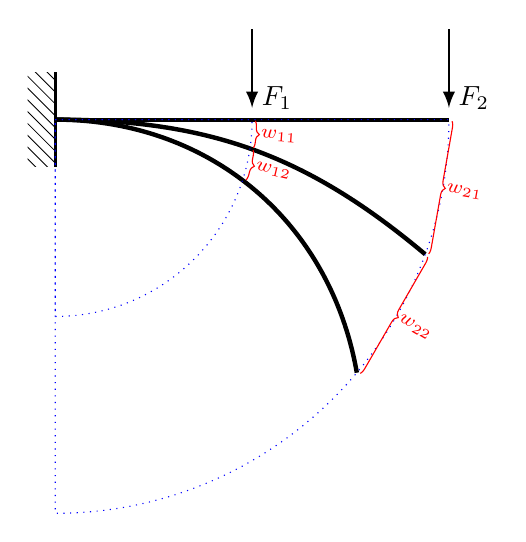
\begin{tikzpicture}[
      inscription/.style={
        decoration = {brace,raise=0.5pt}, % raise moves the brace in the direction it's pointing
        decorate,
        red,
        shorten >=0.8pt, % half the linewidth of ultra thick
        shorten <=0.8pt,
        every node/.style={midway,right,font=\scriptsize}
      },
      arcs/.style={blue,dotted}    
  ]

    %the points
    \point{begin}{0}{0};
    \point{middle}{2.5}{0};
    \point{end}{5}{0};
    %the beam
    \beam{2}{begin}{end};
    %the support
    \support{3}{begin}[-90];
    %the load
    \load{1}{middle}[90];
    \load{1}{end}[90];
    %the inscription of the load
    \notation{1}{middle}{$F_1$};
    \notation{1}{end}{$F_2$};
    %the deflection curves
    \foreach
      [evaluate = {\in = 180 - \angle * 2}] \angle in {20, 40}
    \draw
      [-, ultra thick,name path=defl\angle] (begin) to [out = 0, in = \in] (-\angle : 5) coordinate (ang\angle);
    %circular sector as helplines
    \draw  [arcs,name path=arc1] (begin) -- (middle) arc (0 : -90 : 2.5) -- cycle;
    \draw  [arcs]                (begin) -- (end)    arc (0 : -90 : 5)   -- cycle;
    % find intersections between inner sector and deflections
    \path [
           name intersections={of=defl20 and arc1,by={,D1}}, % first intersection is at "begin", so leave first name empty
           name intersections={of=defl40 and arc1,by={,D2}}];
    %the inscription of the deflection
    \inscription{middle}{D1}{$w_{11}$}
    \inscription{D1}{D2}{$w_{12}$}
    \inscription{end}{ang20}{$w_{21}$}
    \inscription{ang20}{ang40}{$w_{22}$}

  \end{tikzpicture}
\end{document}